\section{Proposed Method}\label{sec:method}
\subsection{Problem Formulation}
Given the observed bounding boxes of a pedestrian over $T{=}15$ frames (0.5\,s at 30\,fps), $\mathbf{X}_{obs}\in\R^{15\times4}$ with $\mathbf{x}_t=(x_1,y_1,x_2,y_2)_t$, the ego-vehicle speed $\mathbf{v}\in\R^{15\times1}$, an ego-motion optical-flow descriptor $\mathbf{F}_{ego}\in\R^{28\times64}$ and a pedestrian optical-flow descriptor $\mathbf{F}_{ped}\in\R^{28\times9}$, the task is to predict the future boxes $\hat{\mathbf{Y}}\in\R^{45\times4}$ for the next 1.5\,s. IDD-PeD additionally provides, for every track, five static scene labels $\mathbf{s}=(s_{int},s_{sig},s_{road},s_{loc},s_{dir})$ (intersection type, signalisation, road type, location type, motion direction) and a per-frame occlusion state $\mathbf{o}\in\{0,1,2,3\}^{15}$.

\subsection{Overview and Major Components}
Fig.~\ref{fig:overall} shows the proposed PACE-Net. The motion inputs are embedded to width $d_{model}{=}32$ (Sec.~\ref{ssec:embed}); a three-layer trajectory encoder produces the trajectory memory $\mathbf{M}_{traj}\in\R^{15\times32}$ (Sec.~\ref{ssec:enc}); a scene-context encoder maps the native IDD-PeD attributes to context tokens and a context vector $\mathbf{c}\in\R^{32}$ (Sec.~\ref{ssec:ctx}); the context is merged into the decoder memory; and a three-layer decoder with three parallel attention sources predicts a residual $\Delta\mathbf{Y}\in\R^{45\times4}$ that is added to the last observed box $\mathbf{x}_T$ repeated 45 times (Sec.~\ref{ssec:dec}).

The design is defined by four major components, each presented in its own subsection with a dedicated figure:
\begin{enumerate}[leftmargin=1.6em,itemsep=1pt,topsep=2pt]
\item \textbf{ROUTE}, adaptive context-memory fusion (Sec.~\ref{ssec:fusion}, Fig.~\ref{fig:fusion}, Algorithm~\ref{alg:fusion}): the context is merged with the trajectory memory by one of three fusion operations (identity, additive, cross-attention) chosen per sample by a learned selector.
\item \textbf{SAGE}, the admission gating mechanism (Sec.~\ref{ssec:gate}, Fig.~\ref{fig:gating}, Algorithm~\ref{alg:gate}): a hard, per-sample gate decides whether the context enters the decoder at all.
\item \textbf{MASC}, memory augmentation (Sec.~\ref{ssec:memory}, Fig.~\ref{fig:gating}b, Algorithm~\ref{alg:gate}): the gated context token is appended to the trajectory memory ($15\to16$ tokens) and exposed to the decoder through a source mask.
\item \textbf{SATIE}, selective weight-parameter sharing (Sec.~\ref{ssec:c4}, Fig.~\ref{fig:sharing}, Algorithm~\ref{alg:share}): only the encoder self-attention projections are tied across layers.
\end{enumerate}
ROUTE, and SAGE with MASC, are two alternative ways of integrating context; both were implemented and evaluated, and the final selected configuration (Sec.~\ref{sec:results}) uses SAGE and MASC together with SATIE. Removing the context pathway and the four components leaves a motion-only configuration (133,700 parameters) that serves as the baseline in the experiments.

\begin{figure*}[t]
\centering
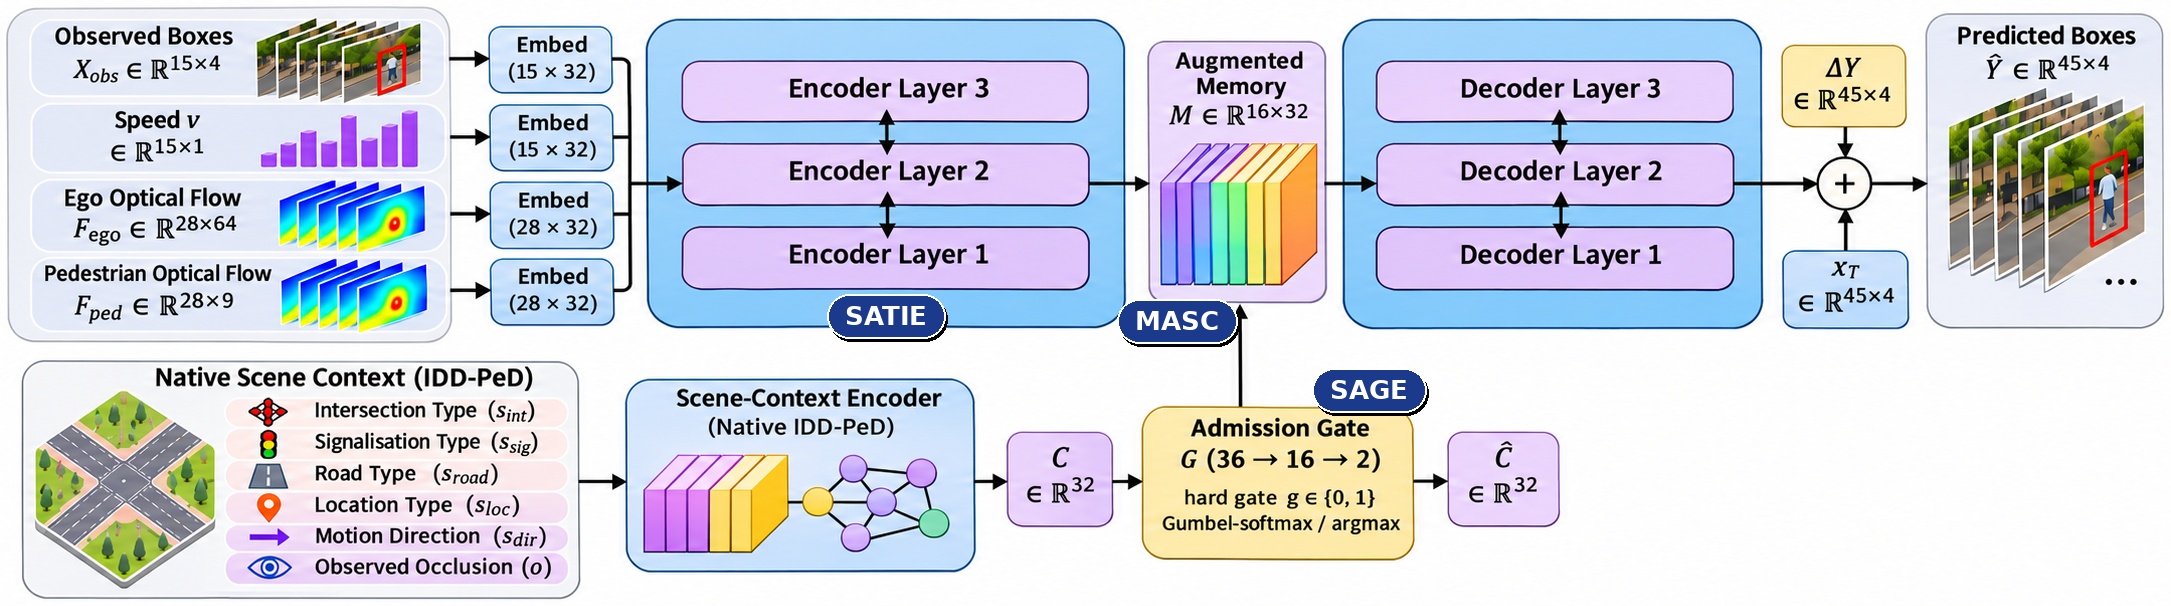
\includegraphics[width=0.97\textwidth]{figures/fig_overall.png}
\caption{Overall architecture of the proposed PACE-Net. Observed boxes and ego speed are embedded to $15{\times}32$ and processed by the three-layer trajectory encoder; the ego-flow and pedestrian-flow embeddings ($28{\times}32$) are consumed by the decoder through attention (Fig.~\ref{fig:decoder}). The five IDD-PeD scene labels and the observed occlusion are encoded into a 32-D context vector, a hard admission gate selects whether the token $\tilde{\mathbf{C}}$ is appended to the memory ($15{\to}16$ tokens), and the decoder output $\Delta\mathbf{Y}$ is added to the last observed box $\mathbf{x}_T$.}
\label{fig:overall}
\end{figure*}

\subsection{Design Rationale}\label{ssec:rationale}
The architecture is organised around five design principles, each of which addresses one of the challenges identified in Sec.~\ref{sec:intro}.
\begin{enumerate}[leftmargin=1.6em,itemsep=1pt,topsep=2pt]
\item \textbf{Separation of motion and context.} Motion evidence (boxes, speed, optical flow) is dynamic and changes at every frame, whereas scene attributes are static for a track. The two are therefore processed in separate pathways and are not mixed inside the encoder, so that the learned motion representation is left undisturbed by the context.
\item \textbf{Late fusion through the decoder memory.} The context pathway outputs a single token that is appended to the memory read by the decoder. Fusion at the memory costs only 5,442 additional parameters (4.07\% of the motion-only configuration) and lets every decoder layer query the context through the same attention mechanism that it uses for motion.
\item \textbf{Conditional admission with a guaranteed fallback.} Scene attributes are informative for some samples and not for others. A hard per-sample gate admits or rejects the token, and rejection removes the token from attention through the source mask, so the decoder then computes exactly what it would compute without context; the context branch can only be used or ignored, never forced.
\item \textbf{Native, interpretable context.} The context pathway consumes the attributes that IDD-PeD already annotates per track (Sec.~\ref{ssec:ctx}) instead of image-level features, which avoids an additional perception network and keeps each input interpretable.
\item \textbf{Selective redundancy removal.} The three encoder layers repeat the same self-attention computation, so only the self-attention projections are shared (Sec.~\ref{ssec:c4}). Source attention, cross attention, feed-forward networks and the decoder serve different roles at different depths and are kept layer-specific.
\end{enumerate}

\subsection{Multimodal Input Embedding}\label{ssec:embed}
Each modality is mapped to $d_{model}{=}32$ by a learned linear embedding, giving $\R^{15\times32}$ for boxes and speed and $\R^{28\times32}$ for the two flow streams (the first row of Fig.~\ref{fig:overall}). The trajectory embedding is followed by positional encoding. The ego and pedestrian flow descriptors use $8{\times}8{=}64$ and $3{\times}3{=}9$ spatial patches respectively, each with two flow channels.

\subsection{Dual-Stream Trajectory Encoder}\label{ssec:enc}
The motion pathway adopts the dual-stream attention block introduced in MTN~\citep{yin2021mtn}. The encoder has $N{=}3$ layers, $h{=}4$ heads, $d_{ff}{=}128$ and dropout $0.1$, and keeps two streams, a trajectory stream $\mathbf{x}$ and a speed-token stream $\mathbf{m}$, both in $\R^{15\times32}$ (Fig.~\ref{fig:encoder}). Layer $l$ computes
\begin{align}
\mathbf{x}' &= \mathbf{x}^{(l-1)} + \Drop\big(\MHA_{self}(\LN(\mathbf{x}^{(l-1)}))\big),\\
\mathbf{m}' &= \mathbf{m}^{(l-1)} + \Drop\big(\MHA_{src}(\LN(\mathbf{m}^{(l-1)}),\mathbf{x}')\big),\\
\mathbf{x}'' &= \mathbf{x}' + \Drop\big(\MHA_{cross}(\LN(\mathbf{x}'),\mathbf{m}')\big),
\end{align}
followed by feed-forward residual blocks that produce $(\mathbf{x}^{(l)},\mathbf{m}^{(l)})$. Source attention lets the speed stream read the trajectory, and cross attention lets the trajectory stream read the speed. The output of the last layer is the trajectory memory $\mathbf{M}_{traj}=\mathbf{x}^{(3)}\in\R^{15\times32}$.

\begin{figure*}[t]
\centering
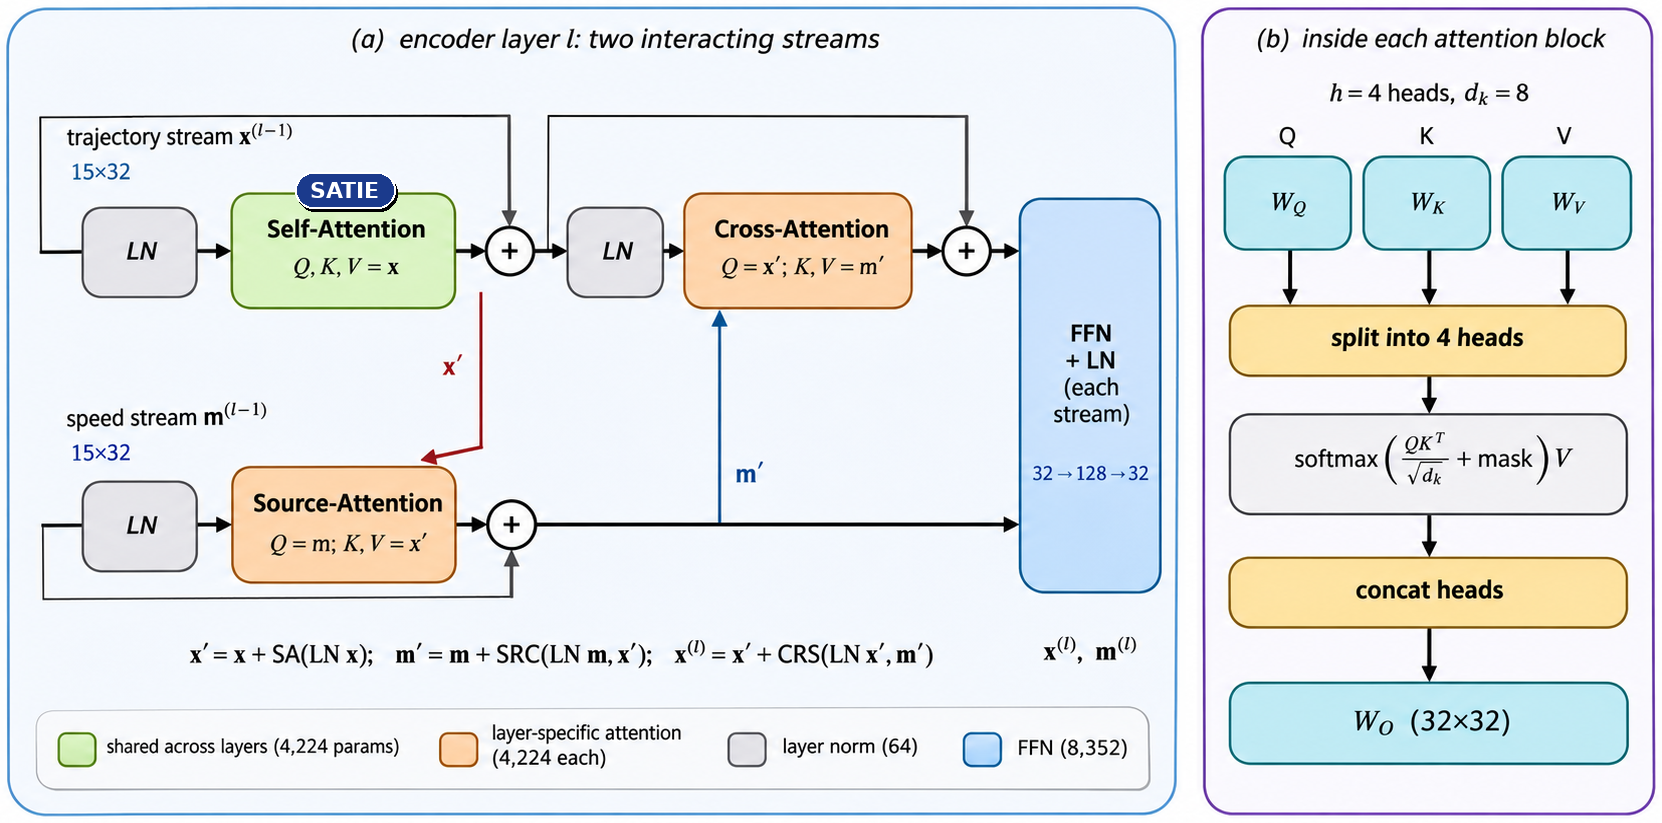
\includegraphics[width=0.85\textwidth]{figures/fig_enc_new.png}
\caption{Dual-stream trajectory encoder layer with shared self-attention. (a)~Layer $l$ updates a trajectory stream $\mathbf{x}$ and a speed stream $\mathbf{m}$ ($15{\times}32$ each) in four steps: self-attention on $\mathbf{x}$ (the module shared across layers, green), source attention in which $\mathbf{m}$ reads the updated trajectory $\mathbf{x}'$, cross attention in which $\mathbf{x}'$ reads the updated speed $\mathbf{m}'$ (both layer-specific, orange), and feed-forward residual blocks. Every sub-layer uses pre-layer-normalisation and a residual connection. (b)~Internal structure of every attention block: query, key and value projections, four heads ($d_k{=}8$), scaled dot-product attention with optional mask, head concatenation and output projection.}
\label{fig:encoder}
\end{figure*}

\subsection{Native Scene-Context Encoding Module}\label{ssec:ctx}
\paragraph{Motivation.} Box and flow history cannot tell whether a pedestrian is at a signalised junction or on an open road. IDD-PeD already annotates such attributes per track, so the proposed model uses them directly, without an additional perception model.

\paragraph{Encoder.} Each categorical field $s_k$, $k\in\{int,sig,road,loc,dir\}$, is embedded into $\R^{16}$ with a learnable table $E_k$ (Fig.~\ref{fig:context}). The observed occlusion sequence is embedded (4 states $\to$16) and mean-pooled over the 15 frames. The six 16-D vectors are concatenated ($6{\times}16{=}96$) and passed through a small MLP:
\begin{align}
\mathbf{u} &= \big[E_{int}(s_{int});\dots;E_{dir}(s_{dir});\ \tfrac1{15}\textstyle\sum_{t}E_{occ}(o_t)\big]\in\R^{96},\\
\mathbf{c} &= W_2\,\Drop\big(\mathrm{GELU}(W_1\,\LN(\mathbf{u})+b_1)\big)+b_2\in\R^{32},
\end{align}
with $W_1\in\R^{32\times96}$ (Fig.~\ref{fig:context}) and $W_2\in\R^{32\times32}$. The context encoder has 4,816 parameters. The fusion variant (Sec.~\ref{ssec:fusion}) additionally keeps the six 16-D vectors as separate tokens, projected to $\R^{6\times32}$ by a shared $16\to32$ layer. Only information available by the end of the observation window is used; time of day is deliberately excluded because it is not an annotated per-track attribute.

\begin{figure*}[t]
\centering
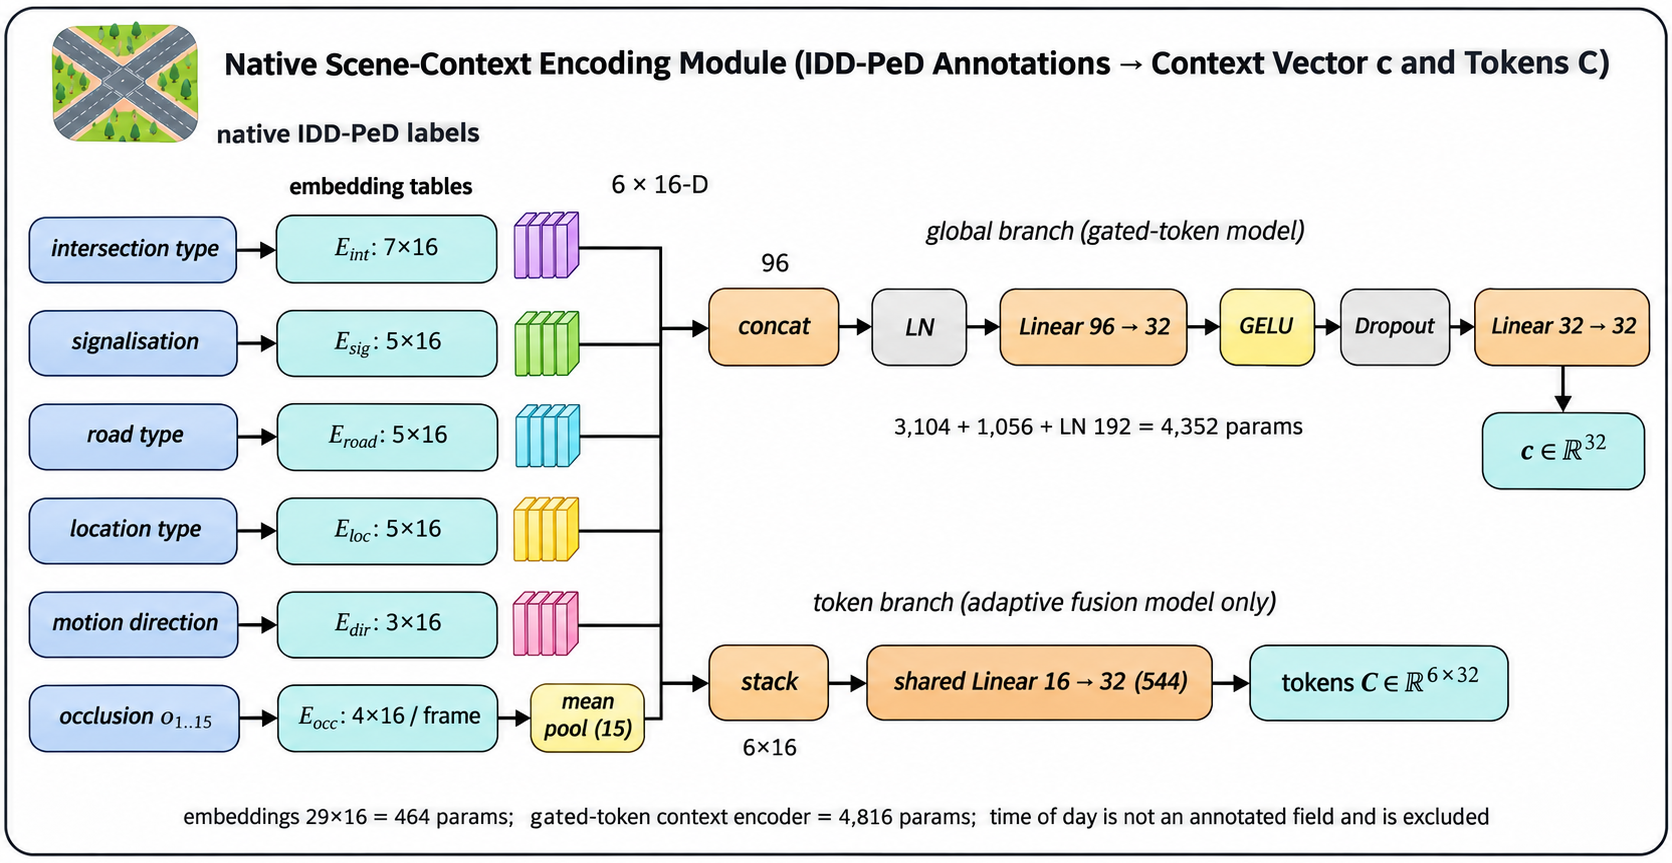
\includegraphics[width=0.85\textwidth]{figures/fig_context_new.png}
\caption{Native scene-context encoding module. Five categorical IDD-PeD labels (with vocabulary sizes 7, 5, 5, 5 and 3, each including an ``unknown'' value) and the 15-frame occlusion sequence (4 states, mean-pooled over time) are embedded to 16-D. The global branch concatenates the six vectors (96-D) and applies layer normalisation and a two-layer MLP to give the context vector $\mathbf{c}\in\R^{32}$ (4,816 parameters in total); the token branch, used only by the adaptive-fusion model, projects the six vectors to context tokens $\mathbf{C}\in\R^{6\times32}$.}
\label{fig:context}
\end{figure*}

\subsection{ROUTE: Routed Operator Unification of Trajectory and Environment}\label{ssec:fusion}
\paragraph{Motivation.} A fixed way of combining context with motion memory cannot suit every pedestrian: for some samples the memory alone suffices, for others a broadcast scene summary helps, and for others the memory should actively query individual scene attributes. ROUTE (Routed Operator Unification of Trajectory and Environment) lets the model choose, per sample, how the context is merged with the trajectory memory, in the spirit of dynamic multimodal fusion~\citep{xue2022dynmm}.

\paragraph{Mechanism.} Let $\mathbf{C}\in\R^{6\times32}$ be the six context tokens and $\mathbf{c}\in\R^{32}$ the global context vector (Sec.~\ref{ssec:ctx}). Three candidate fusions of the trajectory memory are formed (Fig.~\ref{fig:fusion}):
\begin{align}
\mathbf{O}_1&=\mathbf{M}_{traj}, \quad\text{(identity)}\\
\mathbf{O}_2&=\LN\big(\mathbf{M}_{traj}+\mathbf{1}\,\mathbf{c}^\top\big), \quad\text{(additive)}\\
\mathbf{Z}&=\LN\big(\mathbf{M}_{traj}+\MHA(\mathbf{M}_{traj},\mathbf{C},\mathbf{C})\big),\\
\mathbf{O}_3&=\LN\big(\mathbf{Z}+\FFN(\mathbf{Z})\big). \quad\text{(cross-attention)}
\end{align}
A selector
\begin{equation}\boldsymbol{\ell}=W_{s2}\,\mathrm{GELU}\big(W_{s1}[\bar{\mathbf{M}}_{traj};\mathbf{c}]\big)\in\R^{3}\end{equation}
with $W_{s1}\in\R^{32\times64}$ and mean-pooled memory $\bar{\mathbf{M}}_{traj}$ produces one-hot weights $\mathbf{w}$ (hard straight-through Gumbel-softmax in training, $\arg\max$ at inference), and the fused memory $\mathbf{M}_f=\sum_{i=1}^{3}w_i\mathbf{O}_i\in\R^{15\times32}$ replaces $\mathbf{M}_{traj}$ in the decoder (Algorithm~\ref{alg:fusion}). Compared with the motion-only configuration the module adds 20,307 parameters, and all three candidates are computed before selection, so it does not reduce computation.

\begin{figure*}[t]
\centering
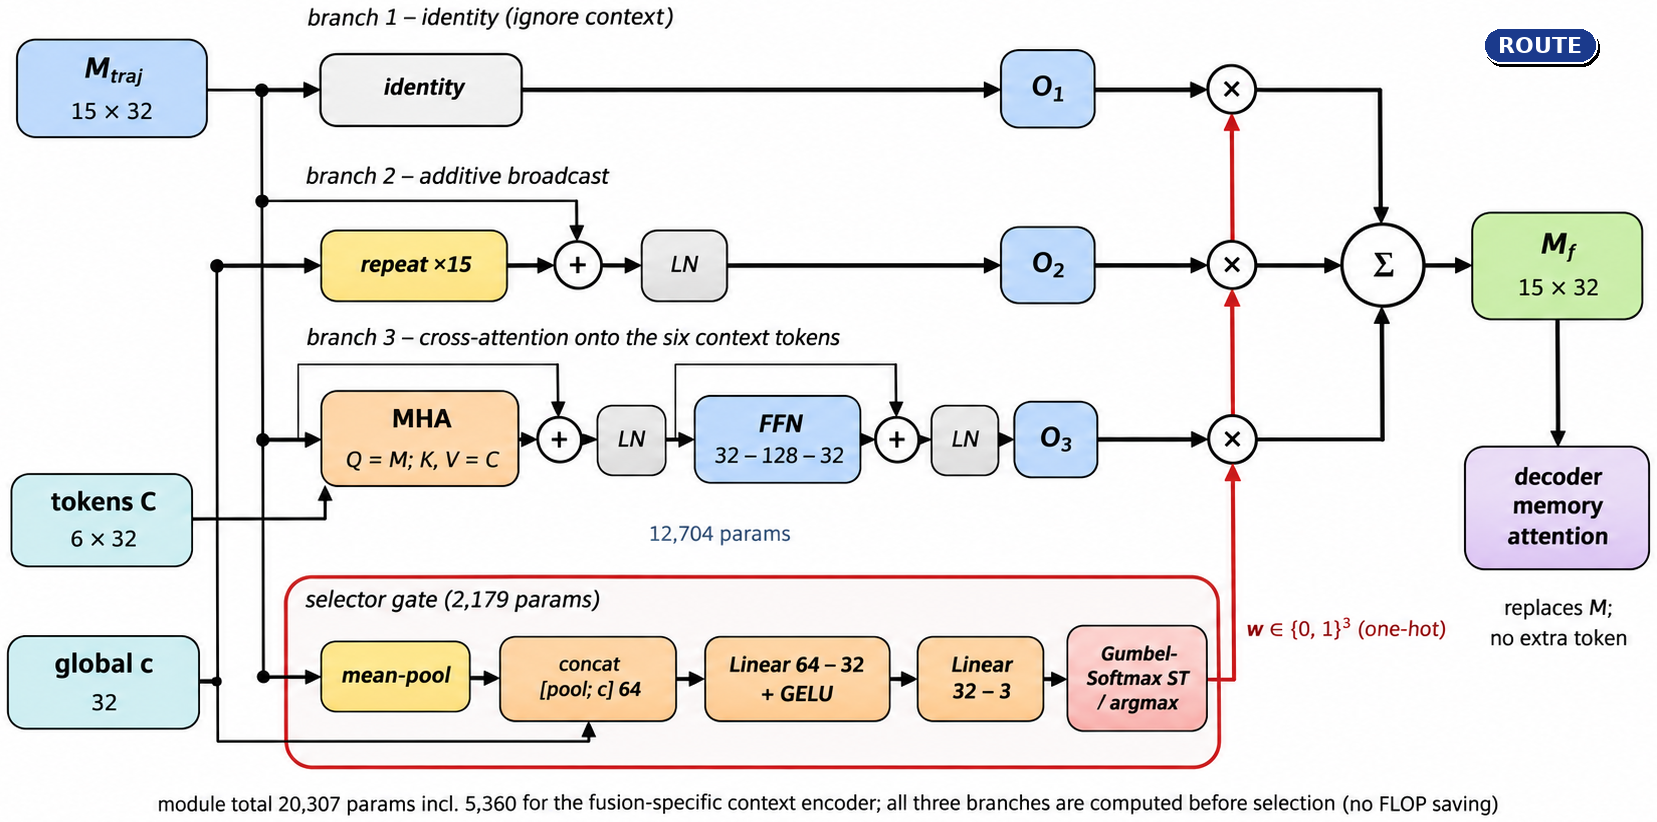
\includegraphics[width=0.85\textwidth]{figures/fig_fusion_new.png}
\caption{ROUTE, the adaptive context-memory fusion module (\textbf{1}). Three fusion operators act on the trajectory memory: identity (branch~1), additive broadcast of the global context followed by layer normalisation (branch~2), and cross-attention onto the six context tokens with a feed-forward block (branch~3). A selector gate on the pooled memory and the global context produces a one-hot weight vector $\mathbf{w}$ (straight-through Gumbel-softmax in training, $\arg\max$ at inference); the weighted sum $\mathbf{M}_f$ replaces the memory read by the decoder.}
\label{fig:fusion}
\end{figure*}

\begin{algorithm}[t]
\caption{ROUTE: adaptive context-memory fusion (forward pass)}\label{alg:fusion}
\begin{algorithmic}[1]
\Require trajectory memory $\mathbf{M}_{traj}\in\R^{15\times32}$, context tokens $\mathbf{C}\in\R^{6\times32}$, global context $\mathbf{c}\in\R^{32}$, mode $\in\{\text{train},\text{eval}\}$
\Ensure fused memory $\mathbf{M}_f\in\R^{15\times32}$
\State $\mathbf{O}_1\gets\mathbf{M}_{traj}$
\State $\mathbf{O}_2\gets\LN(\mathbf{M}_{traj}+\mathbf{1}\mathbf{c}^\top)$
\State $\mathbf{Z}\gets\LN(\mathbf{M}_{traj}+\Drop(\MHA(\mathbf{M}_{traj},\mathbf{C},\mathbf{C})))$
\State $\mathbf{O}_3\gets\LN(\mathbf{Z}+\Drop(\FFN(\mathbf{Z})))$
\State $\boldsymbol{\ell}\gets W_{s2}\,\mathrm{GELU}(W_{s1}[\mathrm{mean}(\mathbf{M}_{traj});\mathbf{c}])$
\If{mode $=$ train}
  \State $\mathbf{w}\gets$ one-hot(GumbelSoftmax$(\boldsymbol{\ell})$) with straight-through gradient
\Else
  \State $\mathbf{w}\gets$ one-hot$(\arg\max\boldsymbol{\ell})$
\EndIf
\State \Return $\sum_{i=1}^{3}w_i\,\mathbf{O}_i$
\end{algorithmic}
\end{algorithm}

\subsection{SAGE: Sample-wise Admission Gate for Evidence}\label{ssec:gate}
\paragraph{Motivation.} Context is not equally informative for every sample, and an uninformative token can distract the decoder. The gate gives the model an explicit, per-sample choice to use or ignore the context, with the motion-only prediction as a guaranteed fallback.

\paragraph{Mechanism.} The gate observes the context vector and the current motion state $\mathbf{x}_T$ (Fig.~\ref{fig:gating}a):
\begin{align}
\boldsymbol{\ell}&=W_{g2}\,\mathrm{GELU}\big(W_{g1}[\mathbf{c};\mathbf{x}_T]+b_{g1}\big)+b_{g2}\in\R^{2},\\
g&=\begin{cases}\text{one-hot}(\mathrm{GumbelSoftmax}(\boldsymbol{\ell}))_2 & \text{training},\\ \arg\max\boldsymbol{\ell} & \text{evaluation},\end{cases}
\end{align}
with $W_{g1}\in\R^{16\times36}$ and $W_{g2}\in\R^{2\times16}$ (626 parameters). The hard straight-through Gumbel-softmax~\citep{jang2017gumbel,bengio2013ste} makes the forward pass discrete while gradients flow through the soft relaxation, so the decision can be learned end to end. The gated token is $\tilde{\mathbf{c}}=g\,\mathbf{c}$.

\begin{figure*}[t]
\centering
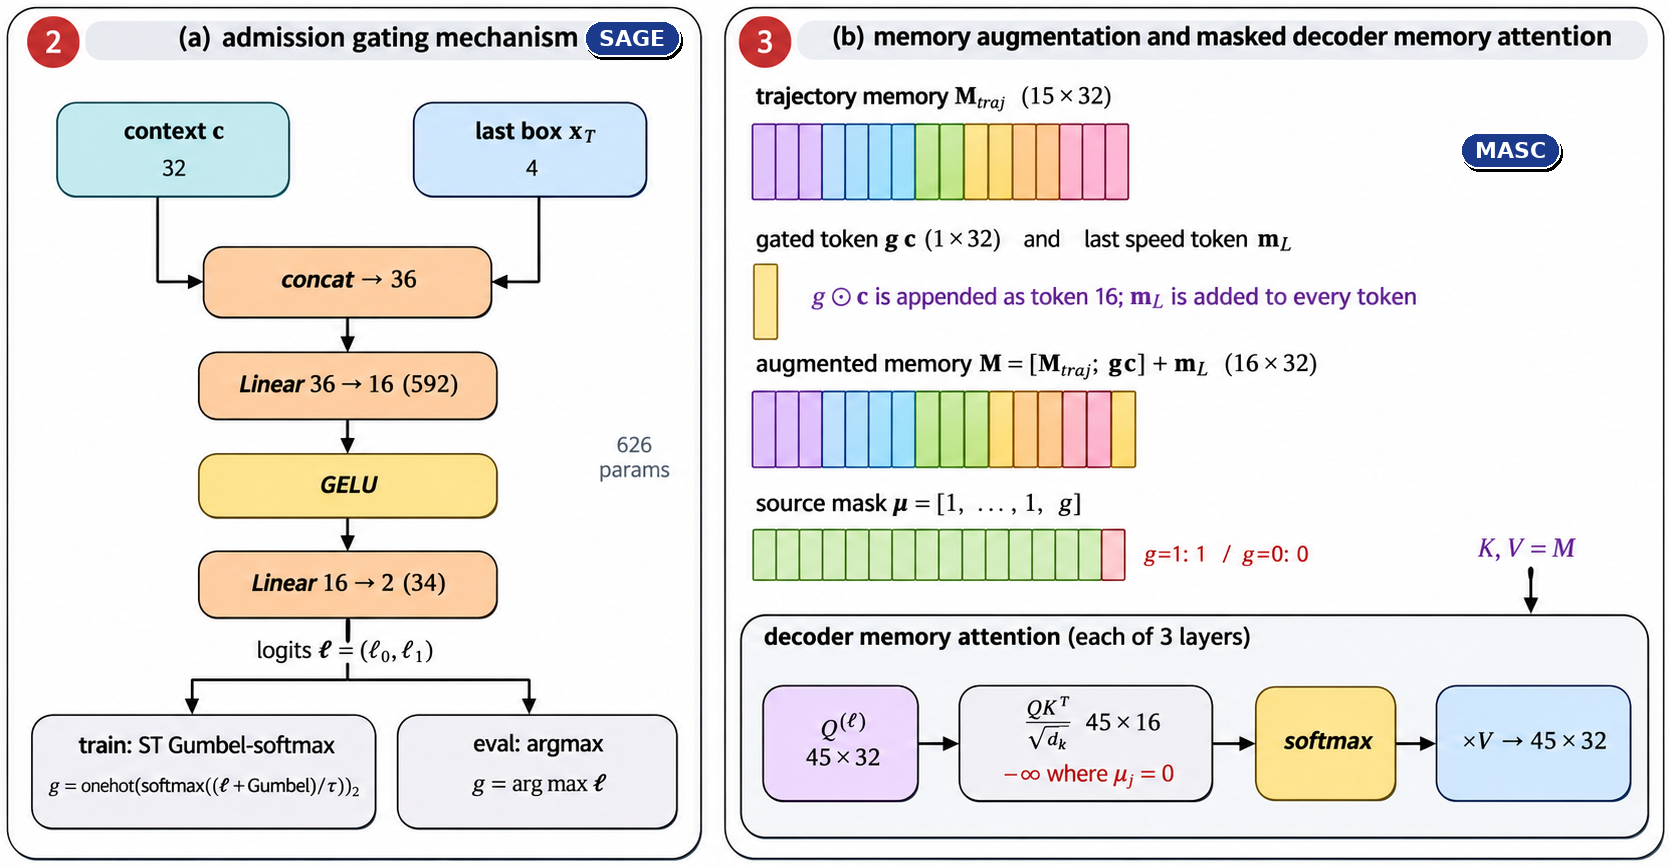
\includegraphics[width=0.85\textwidth]{figures/fig_gate_new.png}
\caption{SAGE admission gating (\textbf{2}) and MASC memory augmentation (\textbf{3}). (a)~The gate concatenates the context vector and last observed box (36-D), applies a two-layer network (626 parameters) and obtains a hard decision $g\in\{0,1\}$ by straight-through Gumbel-softmax (training) or $\arg\max$ (evaluation). (b)~The gated token is appended to the 15 trajectory-memory tokens (16 tokens) and $g$ forms the last entry of the source mask; inside the decoder memory attention, masked keys receive $-\infty$ scores, so a rejected token has zero attention weight.}
\label{fig:gating}
\end{figure*}

\subsection{MASC: Memory Augmentation with Source-masked Context}\label{ssec:memory}
The gated token is appended to the trajectory memory after the encoder (Fig.~\ref{fig:gating}b):
\begin{equation}
\mathbf{M}=\big[\mathbf{M}_{traj};\ g\,\mathbf{c}\big]+\mathbf{m}_L\in\R^{16\times32},\qquad \boldsymbol{\mu}=[\underbrace{1,\dots,1}_{15},\ g],
\end{equation}
where $\mathbf{m}_L$ is the last speed token and $\boldsymbol{\mu}$ is the decoder source mask. When $g{=}0$ the extra token receives \emph{zero attention weight}, so the decoder output equals the output obtained from the 15 motion tokens alone. The context encoder and gate add only 5,442 parameters (4.07\% of the motion-only configuration), and every decoder layer reads the context through the same memory attention it already uses for motion. Algorithm~\ref{alg:gate} summarises the gating and augmentation steps.

\begin{algorithm}[t]
\caption{SAGE admission gating and MASC memory augmentation}\label{alg:gate}
\begin{algorithmic}[1]
\Require motion inputs $(\mathbf{X}_{obs},\mathbf{v},\mathbf{F}_{ego},\mathbf{F}_{ped})$, scene labels $\mathbf{s}$, occlusion $\mathbf{o}$, mode
\Ensure prediction $\hat{\mathbf{Y}}\in\R^{45\times4}$
\State $(\mathbf{M}_{traj},\mathbf{m}_L)\gets\mathrm{Encoder}(\mathbf{X}_{obs},\mathbf{v})$ \Comment{Alg.~\ref{alg:share}}
\State $\mathbf{c}\gets\mathrm{ContextEncoder}(\mathbf{s},\mathbf{o})$ \Comment{$\R^{32}$}
\State $\boldsymbol{\ell}\gets W_{g2}\,\mathrm{GELU}(W_{g1}[\mathbf{c};\mathbf{x}_T])$
\If{mode $=$ train} $g\gets$ hard Gumbel-softmax$(\boldsymbol{\ell})$ \textbf{else} $g\gets\arg\max\boldsymbol{\ell}$ \EndIf
\State $\mathbf{M}\gets[\mathbf{M}_{traj};\,g\,\mathbf{c}]+\mathbf{m}_L$ \Comment{$16\times32$}
\State $\boldsymbol{\mu}\gets[\mathbf{1}_{15},\,g]$ \Comment{source mask}
\State $\Delta\mathbf{Y}\gets\mathrm{Decoder}(\mathbf{M},\boldsymbol{\mu},\mathbf{F}_{ego},\mathbf{F}_{ped})$
\State \Return $\hat{\mathbf{Y}}\gets\Delta\mathbf{Y}+\mathbf{x}_T\mathbf{1}^\top$
\end{algorithmic}
\end{algorithm}

\subsection{SATIE: Self-Attention Tying in the Encoder}\label{ssec:c4}
\paragraph{Motivation.} Cross-layer sharing~\citep{dehghani2019universal,lan2020albert} lowers the parameter count and can regularise training on small data, which is relevant here because the amount of IDD-PeD data used in the experiments is small. Sharing entire layers is harmful when layers play different roles (Sec.~\ref{sec:ablation}), so the question addressed is which sub-modules can be tied safely.

\paragraph{Strategy.} The encoder self-attention repeatedly refines the same trajectory representation, whereas source and cross attention exchange information between two streams whose content changes with depth. Sharing therefore ties only the four self-attention projections,
\begin{equation}
W^{(l)}_{Q,K,V,O}\equiv W^{\star}_{Q,K,V,O},\qquad l=1,2,3,
\end{equation}
by aliasing one module in all three layers (Fig.~\ref{fig:sharing}, Algorithm~\ref{alg:share}). Layer norms, source and cross attention, feed-forward networks and the whole decoder keep their own weights. One attention module has $4\,(32\cdot32+32)=4{,}224$ parameters, so independent layers use $3\times4{,}224=12{,}672$ and shared layers $4{,}224$, a saving of $8{,}448$ parameters (\CAMTN: $139{,}142$; \CAMTNS: $130{,}694$; $-6.07\%$). The tied tensors were verified to have identical object identity and data pointers, and the optimiser receives each shared tensor once. Because the gradient of the shared module is the sum of the three layers' gradients, it is trained by all layers. Sharing reduces parameters and checkpoint size but \emph{not} FLOPs, since the three self-attention calls are still executed.

\begin{figure*}[t]
\centering
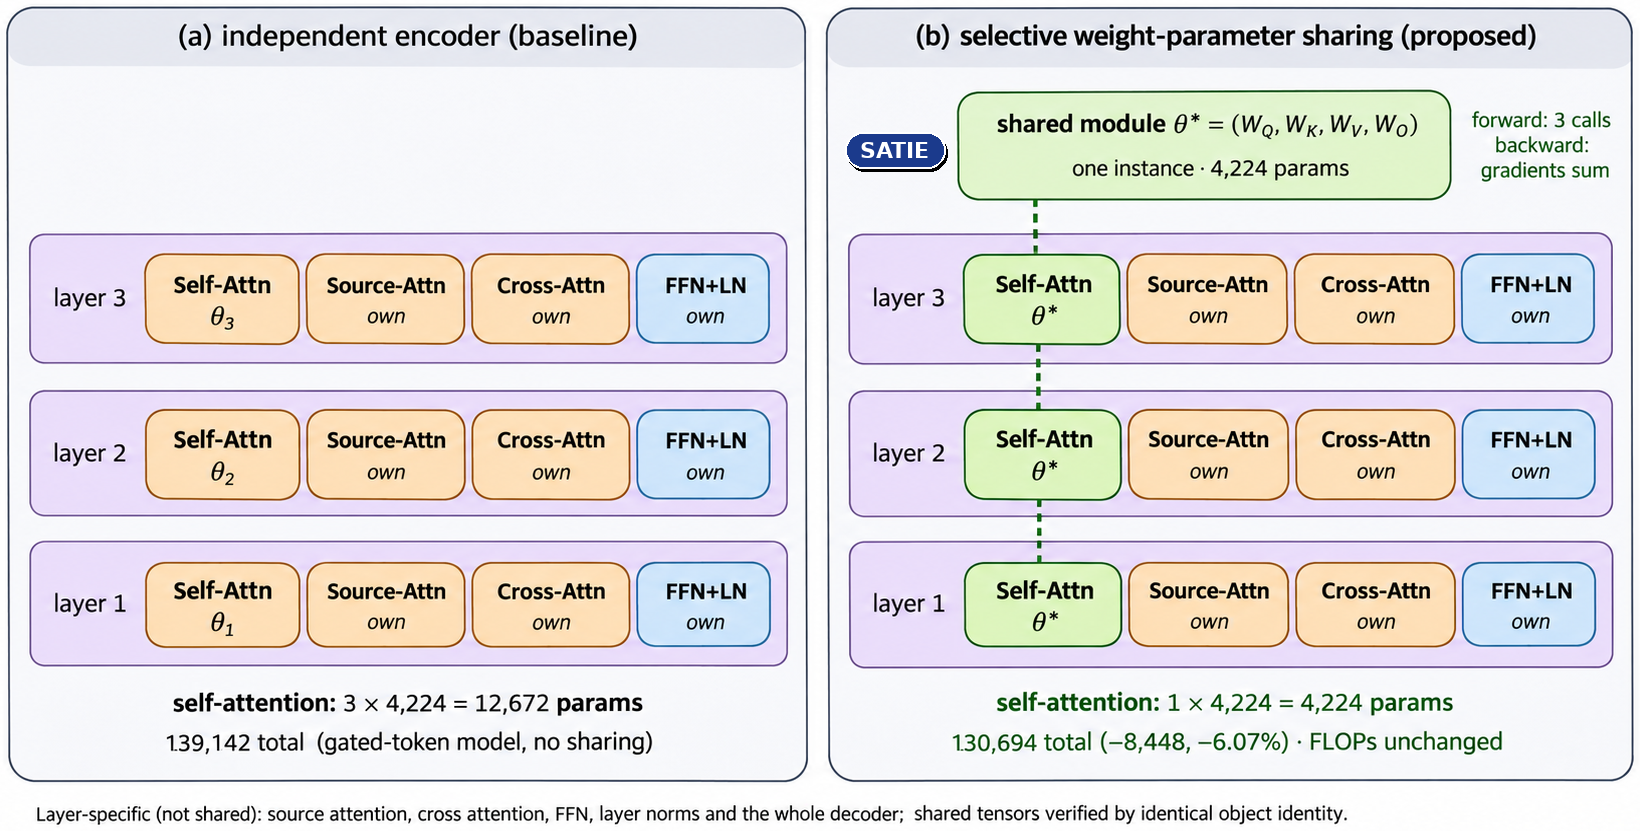
\includegraphics[width=0.85\textwidth]{figures/fig_sharing_new.png}
\caption{SATIE, selective weight-parameter sharing (\textbf{4}). (a)~Independent encoder: each of the three layers owns a self-attention module $\theta_l=(W_Q,W_K,W_V,W_O)$ (12,672 parameters in total). (b)~Proposed: one module $\theta^{\star}$ (4,224 parameters) is aliased in all three layers and receives the summed gradients; source attention, cross attention, feed-forward networks, layer norms and the decoder remain layer-specific. The total parameter count falls from 139,142 to 130,694 ($-6.07\%$) while FLOPs are unchanged.}
\label{fig:sharing}
\end{figure*}

\begin{algorithm}[t]
\caption{SATIE: encoder with selective self-attention sharing}\label{alg:share}
\begin{algorithmic}[1]
\Require embedded trajectory $\mathbf{x}^{(0)}$, speed tokens $\mathbf{m}^{(0)}\in\R^{15\times32}$; layers $N{=}3$
\Ensure trajectory memory $\mathbf{M}_{traj}$, speed stream $\mathbf{m}^{(N)}$
\State \textbf{construct:} $\mathrm{SA}^{\star}\gets\MHA(h{=}4,d{=}32)$ \Comment{single instance, 4,224 params}
\For{$l=1$ \textbf{to} $N$}
  \State $\mathrm{SA}^{(l)}\gets\mathrm{SA}^{\star}$ \Comment{alias, no copy}
  \State $\mathrm{SRC}^{(l)},\mathrm{CRS}^{(l)},\mathrm{FFN}^{(l)},\mathrm{LN}^{(l)}\gets$ new layer-specific modules
\EndFor
\For{$l=1$ \textbf{to} $N$}
  \State $\mathbf{x}'\gets\mathbf{x}^{(l-1)}+\Drop(\mathrm{SA}^{\star}(\LN(\mathbf{x}^{(l-1)})))$
  \State $\mathbf{m}'\gets\mathbf{m}^{(l-1)}+\Drop(\mathrm{SRC}^{(l)}(\LN(\mathbf{m}^{(l-1)}),\mathbf{x}'))$
  \State $\mathbf{x}''\gets\mathbf{x}'+\Drop(\mathrm{CRS}^{(l)}(\LN(\mathbf{x}'),\mathbf{m}'))$
  \State $(\mathbf{x}^{(l)},\mathbf{m}^{(l)})\gets\mathrm{FFN}^{(l)}\text{-residual blocks}(\mathbf{x}'',\mathbf{m}')$
\EndFor
\State \Return $\mathbf{x}^{(N)},\mathbf{m}^{(N)}$ \Comment{gradients of $\mathrm{SA}^{\star}$ sum over layers}
\end{algorithmic}
\end{algorithm}

\subsection{Decoder and Trajectory Prediction}\label{ssec:dec}
Each of the three decoder layers updates its query $Q^{(\ell)}\in\R^{45\times32}$ through three parallel attention branches whose outputs are summed (Fig.~\ref{fig:decoder}):
\begin{multline}
Q^{(\ell+1)}=\FFN\!\Big(A_M(Q^{(\ell)},\mathbf{M})+A_E(Q^{(\ell)},\mathbf{F}_{ego})\\+A_P(Q^{(\ell)},\mathbf{F}_{ped})\Big),
\end{multline}
with $d_{ff}{=}128$. The decoder has no self-attention. A linear head maps the last query to residual offsets $\Delta\mathbf{Y}\in\R^{45\times4}$, and the prediction is $\hat{\mathbf{Y}}=\Delta\mathbf{Y}+\mathbf{x}_T\mathbf{1}^\top$, i.e.\ a residual around constant-position extrapolation (Fig.~\ref{fig:overall}).

\begin{figure}[t]
\centering
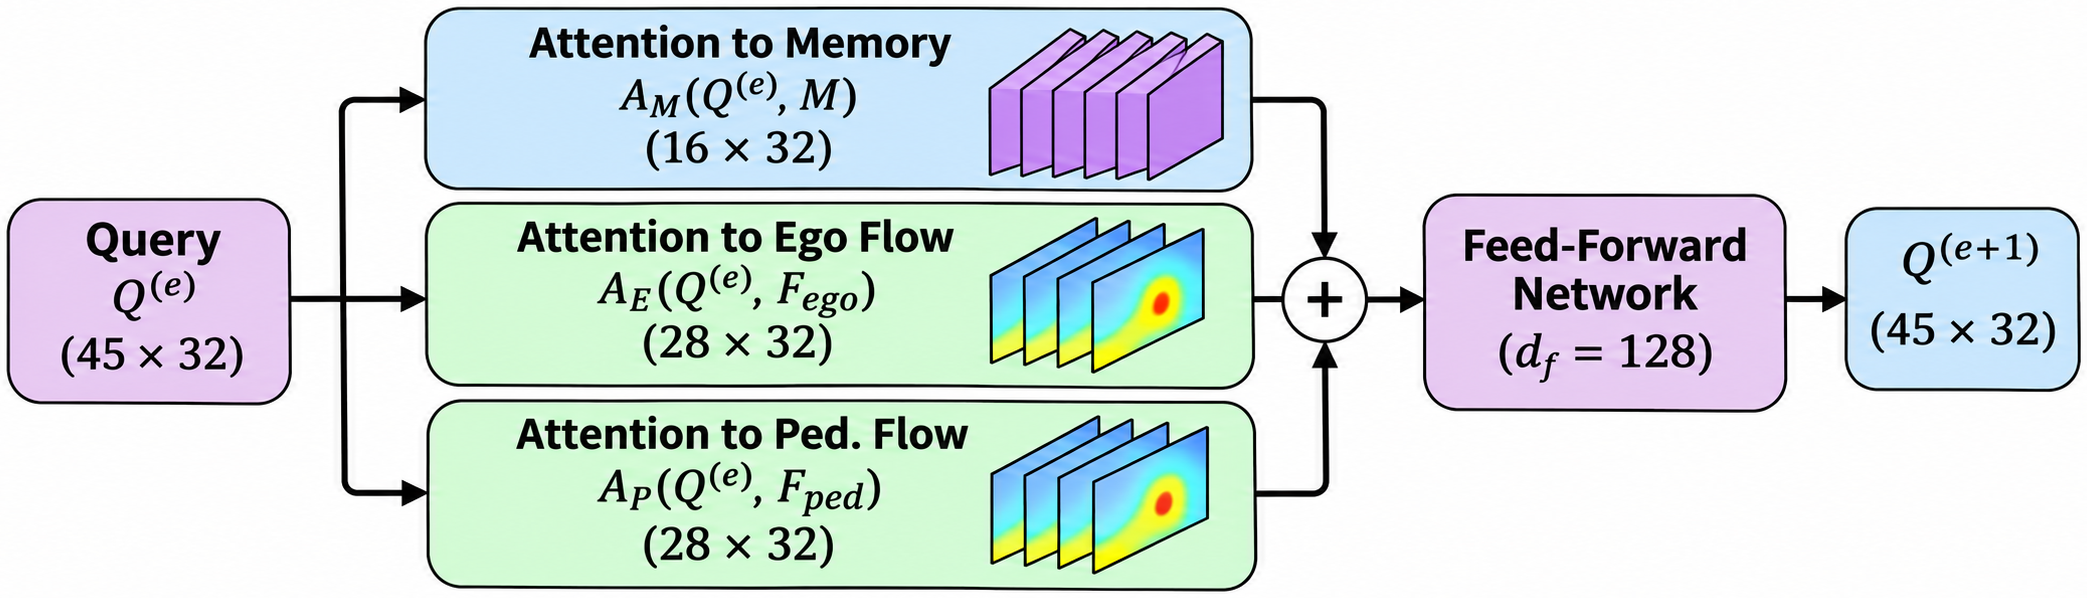
\includegraphics[width=\columnwidth]{figures/fig_decoder.png}
\caption{Decoder layer with three parallel attention sources: the augmented memory ($16{\times}32$), the ego-motion flow and the pedestrian flow (each $28{\times}32$), followed by a feed-forward network ($d_{ff}=128$).}
\label{fig:decoder}
\end{figure}

\subsection{Variants and Training}
\paragraph{Model variants.} Table~\ref{tab:budget} lists the models studied. \CAMTN integrates context through the admission-gated, memory-augmented token without sharing; \CAMTNS adds selective weight-parameter sharing and is the proposed final configuration. \DFMTN replaces the gated token with adaptive context-memory fusion (Sec.~\ref{ssec:fusion}), and \DFMTNS adds sharing to it. The adaptive-fusion models serve as the alternative realisation of the same design and are evaluated under the same protocol (Sec.~\ref{sec:ablation}).

\begin{table}[t]
\centering
\caption{Models studied and their exact parameter counts (measured by instantiating each model).}
\label{tab:budget}
\scriptsize
\begin{tabular}{p{5.6cm}r}
\toprule
Model & Parameters\\
\midrule
MTN (baseline) & 133,700\\
\CAMTN & 139,142\\
\CAMTNS (proposed) & 130,694\\
\DFMTN & 154,007\\
\DFMTNS & 145,559\\
\bottomrule
\end{tabular}
\end{table}

\paragraph{Training.} Every tensor with a matching shape is initialised from the official MTN checkpoint; new modules are randomly initialised and a tied module takes the first layer's weights. Training uses the Adam optimiser~\citep{kingma2015adam} (learning rate $10^{-3}$, batch size 8, one epoch) with an MSE loss between predicted and true 45-step boxes. No auxiliary loss is used.
